\cotefile{104}
\scanpage{2}

\figure{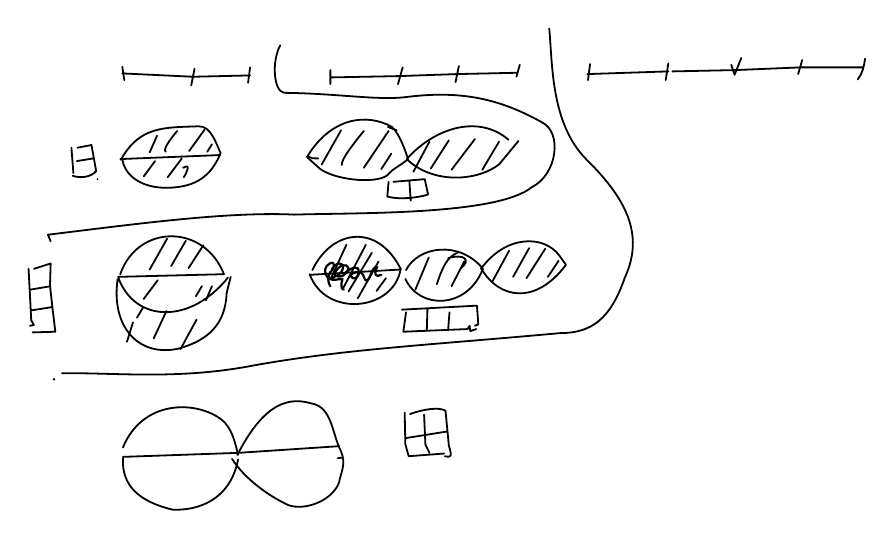
\begin{tikzpicture}[x=.0085cm,y=-.0085cm,line width=.65pt,line cap=round,line join=round]
% Three marked segments across the top.
\draw (227,131)--(333,136)--(418,134) (227,121)--(230,141) (335,124)--(330,149) (418,122)--(415,145);
\draw (538,137)--(641,135)--(727,132)--(818,130) (538,126)--(538,147) (646,122)--(639,147) (730,120)--(725,144) (821,118)--(816,136);
\draw (922,132)--(1043,128) (1049,128)--(1144,126)--(1240,122)--(1334,122) (926,117)--(923,141) (1043,116)--(1039,141) (1137,118)--(1142,133)--(1152,108) (1243,111)--(1237,132) (1337,109) .. controls (1335,122) and (1333,131) .. (1326,140);
% The long dividers pass between the groups of figures.
\draw (463,89) .. controls (450,113) and (453,158) .. (469,160)
 .. controls (552,161) and (610,172) .. (654,166)
 .. controls (736,156) and (793,170) .. (854,204)
 .. controls (885,219) and (877,282) .. (839,301)
 .. controls (787,343) and (583,339) .. (484,342)
 .. controls (384,337) and (240,357) .. (116,372)--(120,382);
\draw (865,64) .. controls (870,116) and (867,205) .. (920,259)
 .. controls (979,317) and (1008,371) .. (978,436)
 .. controls (957,497) and (929,519) .. (882,519)
 .. controls (685,537) and (557,543) .. (420,568)
 .. controls (309,589) and (217,578) .. (137,579);
\fill (125,588) circle[radius=2.2];
% Upright two-cell strip and bisected, hatched oval.
\draw (151,242)--(154,280) (160,242)--(181,238)--(188,277) .. controls (182,284) and (168,289) .. (153,284)
 (159,262)--(184,258);
\fill (190,289) circle[radius=1.45];
\draw (225,260) .. controls (253,209) and (291,212) .. (341,210)
 .. controls (360,209) and (368,238) .. (374,250)
 .. controls (357,292) and (328,301) .. (294,302)
 .. controls (255,302) and (231,284) .. (227,259);
\draw (224,259)--(373,253);
\draw (279,224)--(268,249) (309,217)..controls(299,229)and(287,245)..(292,248)
 (350,215)--(327,247) (361,237)--(354,248)
 (276,262)--(259,285) (316,258)--(295,286) (318,272)..controls(331,264)and(322,282)..(319,286);
% Two joined lenses, above a two-cell strip.
\draw (503,256) .. controls (539,196) and (593,190) .. (630,211)
 .. controls (641,221) and (650,246) .. (654,259)
 .. controls (641,270) and (632,273) .. (626,280)
 .. controls (615,297) and (549,292) .. (523,274)--(503,256);
\draw (504,255)..controls(508,258)and(513,258)..(520,258);
\draw (637,216)--(624,211)
 (652,259) .. controls (696,210) and (761,193) .. (804,230)
 (652,259) .. controls (690,296) and (756,293) .. (790,267)--(819,232);
\draw (554,216)--(525,267) (588,217)..controls(570,239)and(554,260)..(555,268)
 (625,217)--(588,272) (629,251)--(614,274)
 (686,233)--(662,278) (715,231)--(688,273) (754,229)--(719,275) (790,233)--(765,275);
\draw (625,293)--(623,315)..controls(641,320)and(668,317)..(684,312)--(679,289)--(632,293)
 (656,292)--(658,321);
% Three-cell strip, oval and additional lower boundary.
\draw (87,423)--(91,500)--(95,507)--(89,508)
 (95,423)--(120,415)--(119,448)--(123,484)--(127,517)--(93,518)
 (90,454)--(120,449) (92,485)--(123,480);
\draw (224,431) .. controls (250,356) and (349,355) .. (379,431)
 (221,435)--(379,431)
 (221,436) .. controls (246,504) and (329,506) .. (385,436)
 (220,439) .. controls (210,509) and (251,556) .. (312,542)
 .. controls (357,529) and (381,505) .. (383,459)--(389,435);
\draw (294,378)--(268,424) (322,381)--(300,419) (348,388)--(326,422)
 (280,440)--(259,468) (346,449)--(337,464) (361,449)--(352,470)
 (258,481)--(249,496) (243,503)--(234,532) (293,486)--(274,527) (338,499)--(314,543);
% Three horizontal lenses. The first contains heavily retraced ink.
\draw (511,425) .. controls (540,364) and (608,354) .. (643,423);
\draw (643,423) .. controls (633,486) and (531,497) .. (507,431);
\draw (507,432)--(643,424);
\draw (562,387)--(538,439) (591,387)--(556,454) (600,399)--(565,457)
 (610,412)--(579,467) (621,437)--(607,456);
% Dense retraced loops on the chord; no recoverable word or defensible word count.
% Whether an earlier written label was cancelled here remains uncertain.
\draw[line width=.8pt]
 (535,437) .. controls (527,429) and (529,419) .. (537,415)
 .. controls (547,410) and (544,424) .. (537,429)
 .. controls (534,436) and (534,444) .. (538,449)
 (540,424) .. controls (547,412) and (557,413) .. (557,421)
 .. controls (555,432) and (544,436) .. (537,437)
 .. controls (541,442) and (549,438) .. (556,438)
 .. controls (554,446) and (553,453) .. (558,454)
 (544,430) .. controls (551,416) and (563,414) .. (565,422)
 .. controls (565,431) and (551,439) .. (544,432)
 (559,430) .. controls (571,419) and (582,418) .. (580,428)
 .. controls (579,438) and (572,441) .. (568,433)
 .. controls (570,427) and (586,426) .. (587,432)
 .. controls (591,445) and (593,443) .. (598,432)
 .. controls (600,426) and (603,420) .. (608,420)
 .. controls (601,432) and (607,436) .. (614,432);
\draw (651,425)..controls(669,389)and(731,380)..(766,423)
 ..controls(742,484)and(671,484)..(650,438);
\draw (685,406)--(665,454) (728,399)..controls(712,405)and(705,422)..(697,446)
 (714,407)..controls(738,400)and(749,410)..(733,422) (738,412)--(719,449);
\draw (763,423)..controls(800,372)and(857,372)..(880,403)--(890,417)
 ..controls(846,476)and(791,470)..(763,422);
\draw (805,396)--(780,442) (835,392)--(811,435) (859,393)--(831,437) (879,411)--(863,435);
\draw (645,484)--(757,478)--(759,506)--(754,508)
 (651,488)--(647,517)--(743,513)--(746,508)--(747,516)--(756,513) (683,484)--(682,516) (716,488)--(714,513);
% Unshaded pair with one through-line and a four-cell square.
\draw (228,690)..controls(257,619)and(336,619)..(375,648)
 ..controls(390,660)and(395,679)..(400,701);
\draw (400,708) ..controls(391,756)and(356,784)..(303,783)
 ..controls(252,771)and(226,747)..(228,706);
\draw (399,701)..controls(432,637)and(466,611)..(509,624)
 ..controls(541,629)and(540,669)..(554,696)
 ..controls(562,715)and(553,729)..(551,742)
 ..controls(541,770)and(499,785)..(475,776)
 ..controls(447,763)and(411,738)..(391,707);
\draw (228,704)--(400,698)--(551,688);
\draw (556,705)--(549,706);
\draw (649,638)--(650,685)--(655,703)--(708,699)
 (657,640)..controls(676,633)and(700,629)..(710,635)--(715,687)
 ..controls(720,704)and(719,705)..(709,703)
 (678,641)--(680,686)--(686,698) (650,676)--(713,666);
\end{tikzpicture}}

\[
(\text{Ss sets})\,\hookleftarrow\,
(\mathrm{Cat})\,
\unsure{\hookleftarrow|\deleted{\supset}\hookleftarrow}\,
(\deleted{\unsure{\mathrm{Ord}}}\unsure{\text{Préord}|\text{PréOrd}})\,
\supset\,(\mathrm{Ord})\,\supset\,
\left(\overset{\inserted{\text{Maquettes}}}{\deleted{\text{Triang}}}\right)
\]
% The second link is certainly hooked and left-pointing. Its alternative concerns
% only the possible earlier inclusion stroke, not the live arrow's shape.

\[
Fx\longrightarrow Fy
\]

\[
\underset{\smile}{x}\leq\underset{\smile}{y}
\]

% Lower-right margin: six small dark nonlinguistic marks; their origin is uncertain.
\margin{\figure{
\begin{tikzpicture}[x=.025cm,y=-.025cm,line cap=round,line join=round]
\fill (7,5) .. controls (10,4) and (12,3) .. (16,2)
 -- (9,7) .. controls (8,8) and (10,9) .. (10,11)
 .. controls (8,14) and (5,9) .. (7,5) -- cycle;
\fill (9,17) .. controls (12,15) and (13,17) .. (13,18)
 .. controls (17,20) and (13,22) .. (9,21) -- cycle;
\fill (5,27) ellipse[x radius=1.3,y radius=.9];
\fill (2,35) circle[radius=1.3];
\fill (15,35) .. controls (13,36) and (9,38) .. (10,41)
 .. controls (11,43) and (14,45) .. (14,45)
 .. controls (18,46) and (15,42) .. (14,40)
 .. controls (13,38) and (17,36) .. (15,35) -- cycle;
\fill (13,68) ellipse[x radius=2.2,y radius=2.8];
\end{tikzpicture}}}
% archive sheet number: 1
